Since we have constructed different sequences and series, we can move forward into making them more useful for us.  The biggest use for series in our case will be to try and think of functions as a series. Specifically, we may be able to represent a function as a \emph{power series}.  This has many advantages! For one, we can differentiate and integrate a series term by term which simplifies calculations immensely.  Another advantage is the ability to approximate complicated functions.  This is especially useful if one ever plans to use a computer to perform computations.  

\section{Power Series}

Formally, a \boldgreen{power series} is a series with a variable $x$ (typically $x\in \R$ or $z\in \C$) written as
\[
\sum_{n=0}^\infty a_n x^n \qquad \textrm{or} \qquad \sum_{n=0}^\infty a_n z^n.
\]
An immediate question is whether or not this series converges and if that convergence depends on the choice of $x$ we are inputting into the expression.  The tools from the previous chapter allow us to determine this.  But, before that, it is important to get a little intuition on what we're doing here.

A power series is much like a polynomial function
\[
p(x) = a_0 + a_1 x + a_2 x^2 + \cdots + a_N x^N
\]
except for that a power series continues on indefinitely. That is, there is no highest power of $x$ for a power series!  However, if we consider a partial sum of a power series we can realize that as a polynomial. For example, using the series above the $N^\textrm{th}$ partial sum is equivalent to the polynomial above
\[
p(x)=\sum_{n=0}^N a_n x^n.
\]
So, a finite part of a power series is just a polynomial.  In all honesty, this is essentially the idea behind the construction to a power series.  We tend to build these power series as polynomial approximations to functions we already know, or use power series to determine functions in a new way.

\begin{ex}{Partial Sums for Power Series}{partial_sum_power_series}
Consider the power series with $a_n = \frac{1}{n!}$. We write this as
\[
\sum_{n=0}^\infty \frac{x^n}{n!}.
\]
This is an extremely important power series as we will repeatedly.  We can also write this series as
\[
\sum_{n=0}^\infty \frac{x^n}{n!} = 1 + x + \frac{x^2}{2}+\frac{x^3}{6}+\cdots.
\]
Now, let us take the following partial sums and see what the graphs look like. 
\begin{align*}
    \sum_{n=0}^0 \frac{x^n}{n!} &= 1\\
    \sum_{n=0}^1 \frac{x^n}{n!} &= 1+x\\
    \sum_{n=0}^6 \frac{x^n}{n!} &= 1+x+\frac{x^2}{2}+\frac{x^3}{6}+\frac{x^4}{24}+\frac{x^5}{120}+\frac{x^6}{720}.
\end{align*}
Notice how terms of higher powers of $x$ have increasingly smaller contributions to the sum as the denominator gets larger and larger. Below are plots of these.
\begin{figure}[H]
\centering
    \begin{subfigure}[h]{.3\textwidth}
        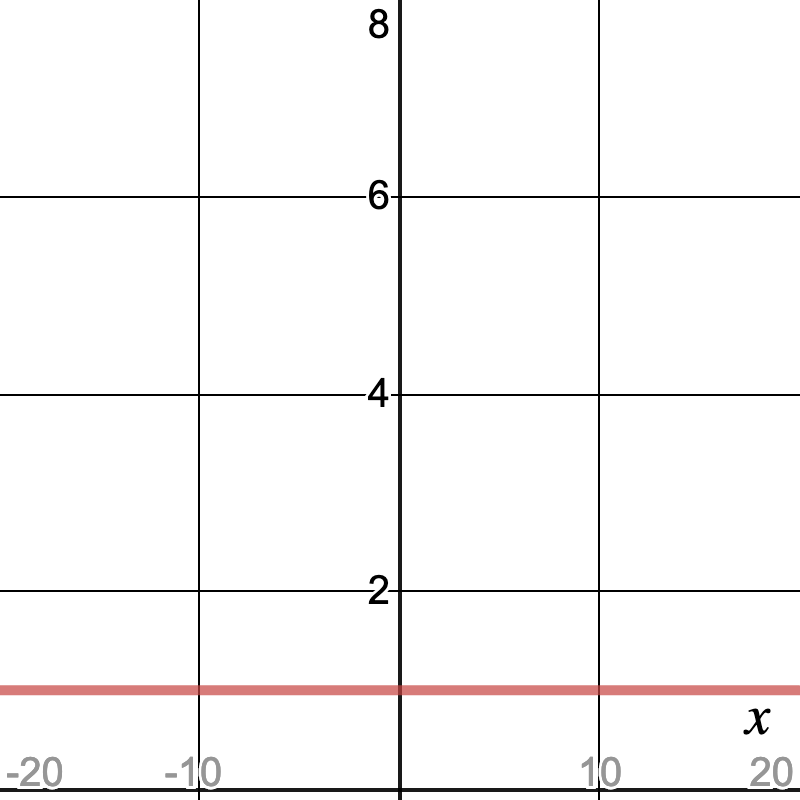
\includegraphics[width=\textwidth]{Figures_Part_3/ex_powseries_N=0.png}
        \caption{Partial sum with $N=0$.}
    \end{subfigure}
    ~
    \begin{subfigure}[h]{.3\textwidth}
        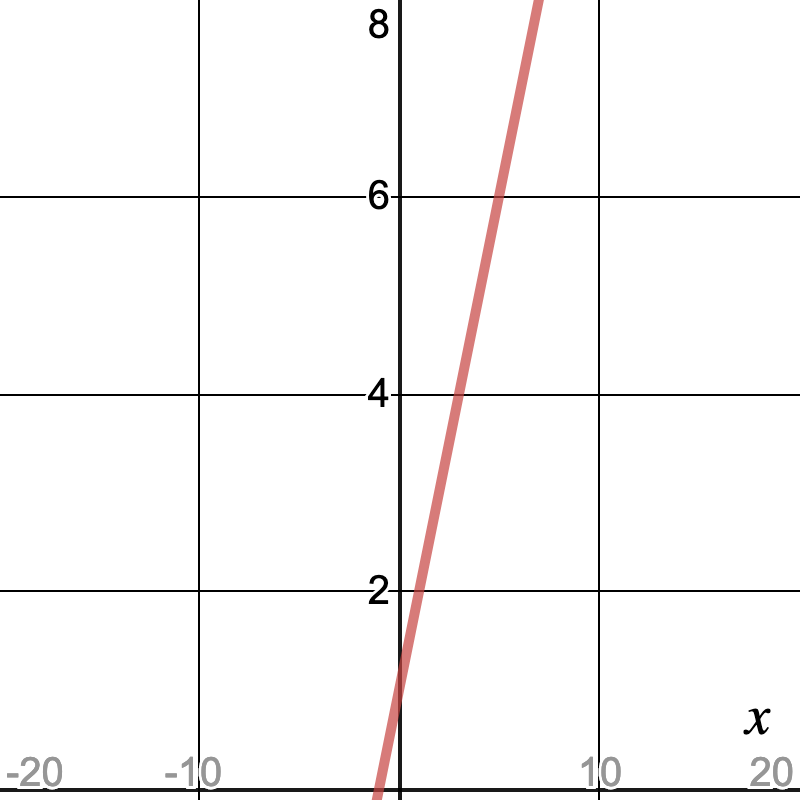
\includegraphics[width=\textwidth]{Figures_Part_3/ex_powseries_N=1.png}
        \caption{Partial sum with $N=1$.}
    \end{subfigure}
    ~
    \begin{subfigure}[h]{.3\textwidth}
        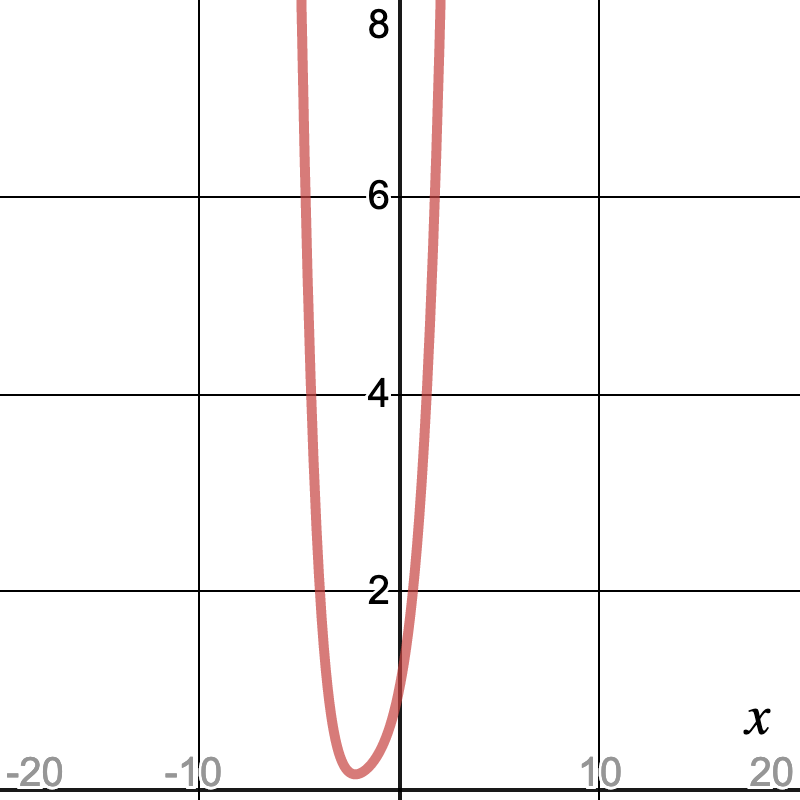
\includegraphics[width=\textwidth]{Figures_Part_3/ex_powseries_N=6.png}
        \caption{Partial sum with $N=6$.}
    \end{subfigure}
\end{figure}
\end{ex}

Before we carry on and see this used in a more applicable way, we just need to know how to talk about convergence of a power series.  A power series is no different than a series, it's just that there is a variable input that may affect convergence.  For example, for large $n$, if $x$ is large, then $x^n$ will be very large.  Thus we must have that the denominator in each term of the power series also grows rapidly. We can test this with the ratio test and determine the values of $x$ (or even $z\in \C$) in which the series converges.

\begin{df}{Radius of Convergence}{radius_of_convergence}
Consider a power series given by $\sum_{n=0}^\infty a_n x^n$.  We define the \boldgreen{radius of convergence} to be the largest value for $|x|$ such that
\[
\lim_{n\to \infty} \left| \frac{a_{n+1}x^{n+1}}{a_n x^n}\right| < 1.
\]
\end{df}

In the above definition we simply used the ratio test to define this. One should also note that this can be generalized slightly to allow for complex valued input $z\in \C$.  All that has to be done is to exchange the absolute value for the modulus.

\begin{ex}{Infinite Radius of Convergence}{radius_of_conv_ex}
Consider again the power series $\sum_{n=0}^\infty \frac{x^n}{n!}$. We wish to find the radius of convergence.  So consider the limit
\begin{align*}
    \lim_{n\to \infty} \left| \frac{\frac{x^{n+1}}{(n+1)!}}{\frac{x^n}{n!}}\right|&= \lim_{n\to \infty} \left| \frac{x}{n+1}\right|\\
    &= 0.
\end{align*}
Since $x$ does not factor into this limit, it does not matter what values of $x$ we plug in. That is, the series will converge no matter our choice for $x$. Fundamentally, this is because $n!$ grows rapdily even compared to $x^n$. Thus, the radius of convergence is infinite.
\end{ex}

\begin{ex}{Finite Radius of Convergence}{radius_of_conv_ex2}
Consider the power series
\[
\sum_{n=1}^\infty \frac{x^n}{n} = x + \frac{x^2}{2}+\frac{x^3}{3}+\frac{x^4}{4}+\cdots.
\]
This power series is similar to a $p$-series for $p=1$.  Hence, we know that if we take $x=1$, the series does not converge.  However, one should note that
\[
\sum_{n=1}^\infty \frac{(-1)^n}{n} = \ln(2).
\]
Given that, we should expect this series to converge for some values of $x$. So, let us use our ratio test 
\begin{align*}
    \lim_{n\to \infty} \left| \frac{\frac{x^{n+1}}{n+1}}{\frac{x^n}{n}}\right| &= \lim_{n\to \infty} \left| \frac{nx}{n+1} \right|\\
    &= |x| \cdot \lim_{n\to \infty} \frac{n}{n+1} \\
    &= |x|.
\end{align*}
Hence, if we want the above limit to be less than one, then we must have $x<1$. Thus the radius of convergence is one.
\end{ex}

One often talks about functions being even or odd by using the following relationships: 
\begin{itemize}
    \item $f(x)$ is \boldgreen{even} if $f(-x)=f(x)$.
    \item $f(x)$ is \boldgreen{odd} if $f(-x)=-f(x)$.
\end{itemize}
This is captured very nicely by a power series. We often say that a power series defines a function and we write
\[
f(x)=\sum_{n=0}^\infty a_n x^n
\]
and we consider the domain of $f(x)$ to be the $x$-values in which the series converges.  

\begin{prop}{Even and Odd Functions}{even_and_odd}
Consider a function $f(x)$ given by a power series so that
\[
f(x) = \sum_{n=0}^\infty a_n x^n
\]
where the series converges. We then say $f(x)$ is \boldgreen{even} if all odd coefficients $a_{2n+1}=0$ and the function is \boldgreen{odd} if all even coefficients $a_{2n}=0$.  

In other words, if $f(x)$ is even, then
\[
f(x)=\sum_{n=0}^\infty a_{2n}x^{2n}
\]
and if $f(x)$ is odd, then
\[
f(x)=\sum_{n=0}^\infty a_{2n+1}x^{2n+1}.
\]
\end{prop}

\section{Taylor Series}

Knowing when a power series converges is helpful, but we have yet to see a way to create relevant power series.  The point of developing these power series is to give a different (and more useful) representation of functions. One way of doing this is called a \emph{Taylor series}.

When first talking of derivatives, we think of tangent line approximations to functions.  Specifically, the derivative is the slope of the tangent line.  Recall, that if we are given a function $f(x)$, we can approximate $f(x)$ with a tangent line passing through the point $a$ by
\[
y = f'(a)(x-a)+f(a).
\]
Now, we should think of the tangent line approximation as the beginning of a power series that approximates $f(x)$.  The intuition to have now is that we could, in some sense, create a tangent quadratic approximation, and a tangent cubic approximation, and so on.  

% Put picture of tangent line, quadratic, and cubic approximation to some function

\begin{figure}[H]
    \centering
    \begin{subfigure}[h]{.3\textwidth}
        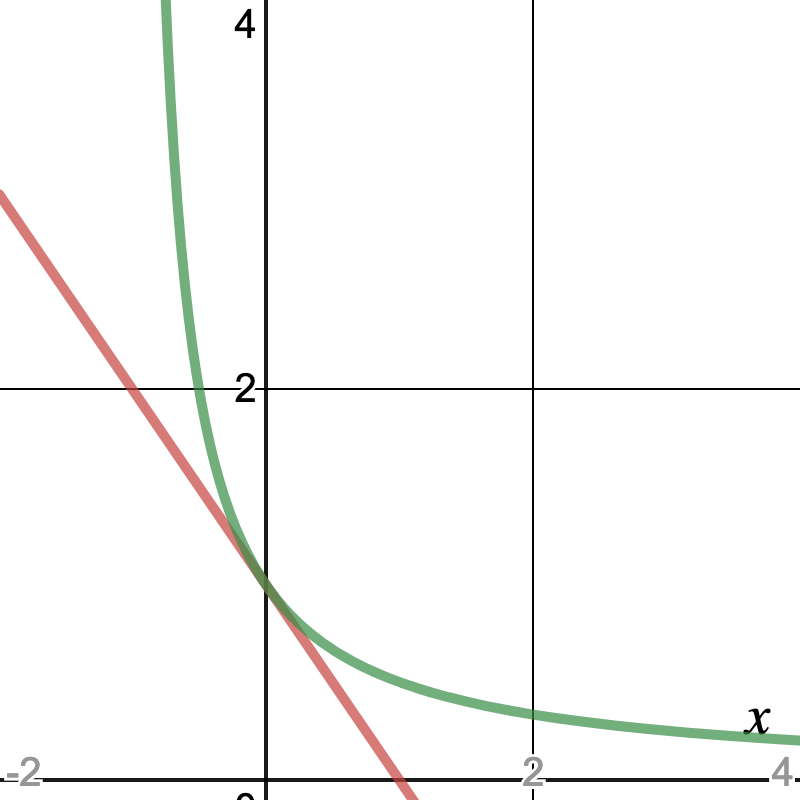
\includegraphics[width=\textwidth]{Figures_Part_3/tangent_line_approx.png}
        \caption{Tangent line approximation to $f(x)=\frac{1}{1+x}$.}
    \end{subfigure}
    ~
    \begin{subfigure}[h]{.3\textwidth}
        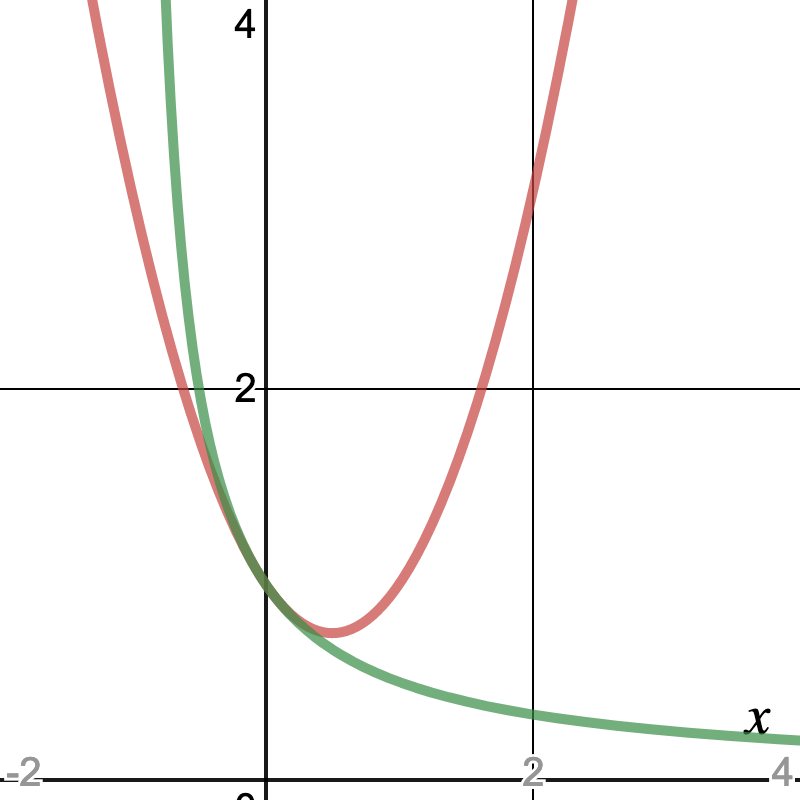
\includegraphics[width=\textwidth]{Figures_Part_3/tangent_quad_approx.png}
        \caption{Tangent quadratic approximation to $f(x)=\frac{1}{1+x}$.}
    \end{subfigure}
    ~
    \begin{subfigure}[h]{.3\textwidth}
        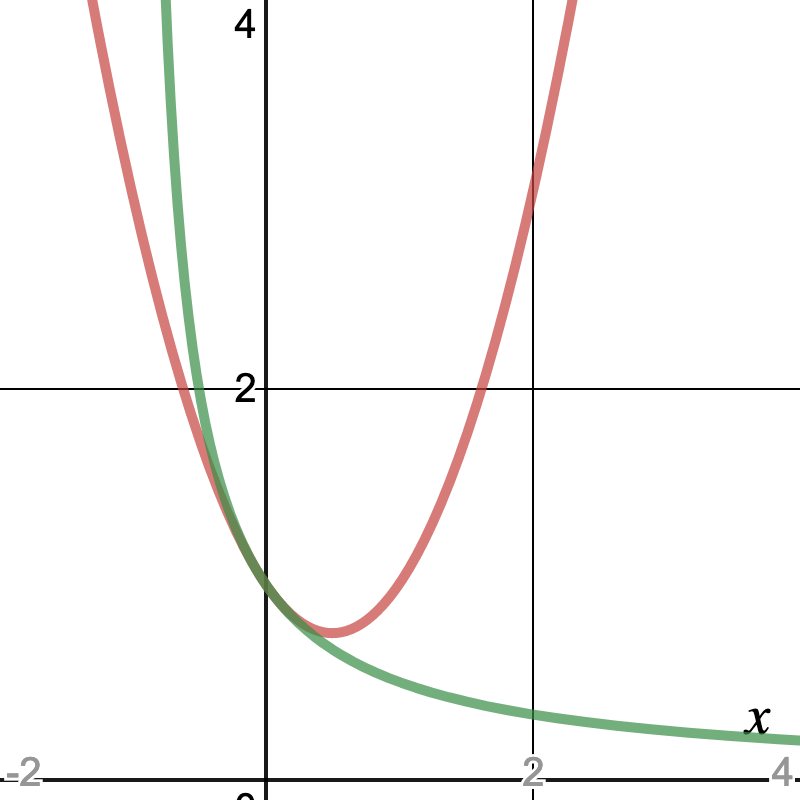
\includegraphics[width=\textwidth]{Figures_Part_3/tangent_quad_approx.png}
        \caption{Tangent cubic approximation to $f(x)=\frac{1}{1+x}$.}
    \end{subfigure}
\end{figure}

Let us think for a moment about how we may construct a series that gives us the above approximations and more.  If we are to pick a point $x=a$ to build our approximation from, then the approximation should have the same value as the function at the point $a$.  So, the zeroth order approximation (i.e., the zeroth term in the series we're building) should be $f(a)$.  Notice that $f(a)$ occurs in the tangent line approximation.  Next, if we take a first order approximation, this should give us an equation for a line. The best approximation around $a$ to the function $f(x)$ with a line would be the tangent line approximation.  The first derivative tells us the information about the slope.  Now, notice the tangent line approximation above contains the zeroth order approximation as well. Functions also tend to have some curvature to them and this is captured nicely by the second derivative of the function at the point $a$.  Now we can add in this second derivative information to get a tangent quadratic
\[
f(a)+f'(a)(x-a)+\frac{f''(a)}{2!}(x-a)^2.
\]
This would be our second order approximation. Similarly, we can build the tangent cubic (or third order approximation) by
\[
f(a)+f'(a)(x-a)+\frac{f''(a)}{2!}(x-a)^2+\frac{f'''(a)}{3!}(x-a)^3.
\]
Taking this pattern in mind, we can create the $N^\textrm{th}$ order approximation to be
\[
f(a)+f'(a)(x-a)+\frac{f''(a)}{2!}+\cdots + \frac{f^{(N)}(a)}{N!}(x-a)^N.
\]
As it turns out, for many functions we can continue this process infinitely and create a power series that exactly matches the function we started with.

\begin{df}{Taylor Series}{taylor_series}
Given a function $f(x)$ that is \emph{analytic} in a region around the point $x=a$, we can construct the \boldgreen{Taylor series centered at $x=a$}
\[
\sum_{n=0}^\infty \frac{f^{(n)}(a)}{n!}(x-a)^n
\]
which is equal to the function $f(x)$ (on a sufficiently small interval $(a-\epsilon, a+\epsilon)$. If we let $a=0$, we call this the \boldgreen{Maclaurin series}.  
\end{df}

Though the definition above only guarantees that the Taylor series is equal to the function on a small interval, many functions we care about will satisfy
\[
f(x)=\sum_{n=0}^\infty \frac{f^{(n)}(a)}{n!}(x-a)^n
\]
for large intervals or even all real numbers.  

\begin{ex}{Maclaurin Series for $e^x$}{maclaurin_exp}
Consider the function $f(x)=e^x$.  We consider constructing the Maclaurin series (Taylor series centered at $x=0$) for $e^x$ by
\[
\sum_{n=0}^\infty \frac{f^{(n)}(0)}{n!}x^n.
\]
Now, note that $f^{(n)}(x)=e^x$ and so $f^{(n)}(0)=1$ for every $n$.  Hence we have that the Maclaurin series for $e^x$ is
\[
\sum_{n=0}^\infty \frac{x^n}{n!}.
\]
It turns out that we have
\[
e^x = \sum_{n=0}^\infty \frac{x^n}{n!}
\]
for all real numbers.
\end{ex}

It's nice to see a few examples of this construction, so let us consider another example.

\begin{ex}{Maclaurin Series for $\ln(1+x)$}{maclaurin_ln}
Consider the function $f(x)=\ln(1+x)$.  We can build the Maclaurin series for $f(x)$ using
\[
\sum_{n=0}^\infty \frac{f^{(n)}(0)}{n!}x^n.
\]
Now we should take a few derivatives of $f(x)$ to see the pattern we need.
\begin{align*}
    f(x)&= \ln(1+x) ~\implies~ f(0)=0\\
    f'(x)&=\frac{1}{1+x} ~\implies~ f'(0)=1=0!\\
    f''(x)&= -\frac{1}{(1+x)^2} ~\implies~ f''(0)=-1=-1!\\
    f'''(x)&= \frac{2}{(1+x)^3} ~\implies~ f'''(0)=2=2!\\
    f^{(4)}(x)&= -\frac{6}{(x+1)^4} ~\implies~ f^{(4)}(0)=-6=-3!.
\end{align*}
So we have that $f^{(n)}(0)=(-1)^{n-1}(n-1)!$ for $n\geq 1$. So our series takes the form
\[
\sum_{n=1}^\infty \frac{(-1)^{n-1}(n-1)!}{n!}x^n = \sum_{n=1}^\infty \frac{(-1)^{n-1}}{n}x^n.
\]
It turns out here that we have 
\[
\ln(1+x)=\sum_{n=1}^\infty \frac{(-1)^{n-1}(n-1)!}{n!}x^n = \sum_{n=1}^\infty \frac{(-1)^{n-1}}{n}x^n
\]
for $x\in (-1,1)$.  
\end{ex}

\begin{exercise}
Determine the radius of convergence of the power series for $\ln(1+x)$.
\end{exercise}

Taylor series granted us the ability to create power series representations of functions.  However, not all functions have a useful Taylor series.  The prototypical example is the \emph{bump} function
\[
f(x) = \begin{cases} e^{-\frac{1}{x^2}} & \textrm{if $\neq 0$}\\ 0 & \textrm{if $x=0$} \end{cases}.
\]
If one computes $f^{(n)}(0)$ they find that it is zero for each $n$. So the Taylor series centered at $0$ is the zero series! Even though the function is infinitely differentiable at $x=0$, it isn't analytic there.

\section{Operations with Power Series}
% ADD IN POWER SERIES SUBSTITUTION like $e^{x^2}$ into the series for $e^x$.
Since we created power series to essentially be polynomials, we hope to gain some of the nice properties of polynomials as well.  Even though the sums are infinite, it turns out that we still get integral and derivative properties like the sum and product rule.  So, given a power series representation for a function (where the $x$ are within the radius of convergence)
\[
f(x)=\sum_{n=0}^\infty a_n x^n,
\]
we want to consider
\[
\frac{d}{dx} f(x) \qquad \textrm{and} \qquad \int f(x) dx.
\]
Since the derivative and integral are \emph{linear operators} (more on this later) we know they satisfy the sum and constant multiple rules which leads us to
\[
\frac{d}{dx} f(x) = \frac{d}{dx} \sum_{n=0}^\infty a_n x^n = \sum_{n=0}^\infty a_n \frac{d}{dx} x^n
\]
and
\[
\int f(x) dx = \int \sum_{n=0}^\infty a_nx^n dx = \sum_{n=0}^\infty a_n \int x^n dx.
\]

Let us concentrate first on differentiating the power series.  So, we have 
\begin{align*}
\frac{d}{dx} \sum_{n=0}^\infty a_nx^n&=\frac{d}{dx} \left(a_0 + a_1x + a_2 x^2 + a_3 x^3 \cdots\right)\\
&= a_1 + 2a_2x+3a_3x^2+\cdots.
\end{align*}
Notice now that the zeroth term in the series has been deleted, and what we have is then
\[
\boxed{\frac{d}{dx} \sum_{n=0}^\infty a_n x^n = \sum_{n=1}^\infty na_n x^{n-1}.}
\]
One could rearrange this series and continue starting it at zero.  We simply have to make sure that the series remains the same after this process.  So, equivalently, one could write
\[
\frac{d}{dx} \sum_{n=0}^\infty a_n x^n = \sum_{n=0}^\infty (n+1)a_{n+1} x^n.
\]

\begin{exercise}
    Verify that the reindexing above makes sense.  
\end{exercise}

\begin{exercise}
    How can we compute second derivatives of a power series? What terms do we lose? What about $n^\textrm{th}$ derivatives?
\end{exercise}

And now we turn to integration. Approaching this in the same way we have
\begin{align*}
    \int \sum_{n=0}^\infty a_n x^n &= \int \left( a_0 +a_1x+a_2x^2+a_3x^3+\cdots\right)dx\\
    &= C+a_0x+\frac{a_1}{2}x^2+\frac{a_2}{3}x^3+\frac{a_3}{4}x^4+\cdots.
\end{align*}
Thus we have that
\[
\boxed{\int \sum_{n=0}^\infty a_n x^n dx = C + \sum_{n=0}^\infty \frac{a_n}{n+1} x^{n+1},}
\]
where $C$ is the undetermined constant from integration.

\begin{exercise}
    Try integrating a power series twice.
\end{exercise}

\begin{ex}{Differentiating and Integrating $e^x$}{diff_int_ex}
We have the power series representation for $e^x$ given by
\[
e^x = \sum_{n=0}^\infty \frac{x^n}{n!}.
\]
Now, if we consider
\begin{align*}
    \frac{d}{dx} \sum_{n=0}^\infty \frac{x^n}{n!} &= \sum_{n=1}^\infty  \frac{nx^{n-1}}{n!}\\
    &=\sum_{n=1}^\infty \frac{x^{n-1}}{(n-1)!}\\
    &= \sum_{n=0}^\infty \frac{x^n}{n!}\\
    &=e^x,
\end{align*}
which is what we expect.  Similarly,
\begin{align*}
    \int \sum_{n=0}^\infty \frac{x^n}{n!} &= C+\sum_{n=0}^\infty \frac{x^{n+1}}{(n+1)n!}\\
    &= C+\sum_{n=0}^\infty \frac{x^{n+1}}{(n+1)!}.
\end{align*}
Now, this should be equal to $e^x+C$ for some undetermined constant $C$. So notice that if we replace $C=D+1$ (which is fine, since $C$ is undetermined), we have
\begin{align*}
    \int \sum_{n=0}^\infty \frac{x^n}{n!} &= D+1+\sum_{n=0}^\infty \frac{x^{n+1}}{(n+1)!}\\
    &= D + 1 + x+\frac{x^2}{2}+\frac{x^3}{3!}+\cdots\\
    &= D+ \sum_{n=0}^\infty \frac{x^n}{n!}\\
    &= D+e^x,
\end{align*}
which does give us what we expect.
\end{ex}

\begin{remark}
With integration and differentiation of series, one just has to be very careful. It often helps to write out part of the series (as shown above) to analyze the problem further.  This is why we begin with examples of functions we already understand well!
\end{remark}

\section{Approximation with Power Series}
A big application of power series is the ability to approximate functions with polynomials.  We did indeed begin developing the Taylor series in order to approximate functions in this way after all.  If we have a function $f(x)$ that is $N$ times differentiable, then we can approximate $f(x)$ around the value $x=a$ as
\[
f(x)\approx \sum_{n=0}^N \frac{f^{(n)}(a)}{n!}(x-a)^n = f(a)+f'(a)(x-a)+\frac{f''(a)}{2!}(x-a)^2+\cdots + \frac{f^{(N)}(a)}{N!}(x-a)^N
\]
which is just a truncation of the Taylor series for $f$. Of course, we may not have that the power series is totally useful (see the end of Section 6.2), but we also have relaxed the assumption that we need to take infinitely many derivatives of $f(x)$.  In fact, it turns out that having two derivatives tends to be plenty as a quadratic approximation works remarkably well.

\begin{df}{Order of an Approximation}{order_of_approx}
Given an approximation of $f(x)$ about the point $x=a$
\[
f(x) \approx \sum_{n=0}^N \frac{f^{(n)}(a)}{n!}(x-a)^n,
\]
we refer to the \boldgreen{order of the approximation} as the highest power of $x$ that appears. In the above case, we would say that this is an $N^\textrm{th}$ order approximation of $f(x)$. 
\end{df}

It's worth seeing some examples of different orders of approximations to see just how well they fare for different functions.  

\begin{ex}{Approximating $e^x$}{approx_ex_order}
Consider the function $e^x$ which has the Taylor series centered at $a=0$ given by
\[
e^x = \sum_{n=0}^\infty \frac{x^n}{n!}.
\]
Then we have the approximations
\begin{align*}
    0^\textrm{th}:~e^x&\approx 1\\
    1^\textrm{st}:~e^x&\approx 1+x\\
    2^\textrm{nd}:~e^x&\approx 1+x+\frac{x^2}{2}.
\end{align*}
\end{ex}

\begin{ex}{How Accurate are Approximations of $\sin(x)$}{approx_sinx}
Consider the function $\sin(x)$ which has the Taylor series centered at $a=0$ 
\[
\sin(x) = \sum_{n=0}^\infty \frac{(-1)^n x^{2n+1}}{(2n+1)!}.
\]
Then we can consider the approximations
\begin{align*}
    0^\textrm{th}:~\sin(x)&\approx 0\\
    1^\textrm{st}:~\sin(x)&\approx x\\
    2^\textrm{nd}:~\sin(x)&\approx x\\
    3^\textrm{rd}:~\sin(x)&\approx x-\frac{x^3}{3!}.
\end{align*}
Due to the fact that $\sin(x)$ is an odd function, we have that the even order approximations don't do any better than the previous odd order approximation.  We can compare the accuracy of the first and third order approximations to the real function values. 
    \begin{table}[H]
        \centering
        \renewcommand{\arraystretch}{1.5}
        \begin{tabular}{c|c|c|c}
            Input & True Value & 3$^\textrm{3rd}$ Order Approx.\\
            \hline
            $x$ & $\sin(x)$ & $x-\frac{x^3}{3!}$\\
            \hline
            0.001 & $\approx 0.000999999$ & $0.0009999998\overline{3}$\\
            \hline
            0.01 &  $\approx 0.00999983$ & $0.0099998\overline{3}$\\
            \hline
            0.1 &  $\approx 0.0998334$ & $0.0998\overline{3}$\\
            \hline
            0.5 & $\approx 0.479426$ & $0.4791\overline{6}$\\
            \hline
            1.0 & $\approx 0.841471$ & $0.8\overline{3}$
        \end{tabular}
        \label{tab:sin_approx}
    \end{table}
    Note that the leftmost column is also the first order approximation. One can see that to six significant digits, the third order approximation does a great job even up to $\sin(1)$.  The upshot is that the third order approximation is far easier to work with than the function $\sin(x)$ itself (which we tend to use the whole series for).
\end{ex}

Since these approximations can do such a great job, it's worthwhile to see how we can use these approximations in practice

\begin{ex}{The Pendulum Problem}{pendulum}
Consider a pendulum system mounted to a frictionless pivot with a bob of mass $m$ a distance $L$ from the pivot. If we pull the bob up by an angle $\theta$, the force if gravity $mg$ is directed downward and thus causes a force of $-mg\sin\theta$ on the bob.  We can draw this system out as follows:
\begin{figure}[H]
    \centering
    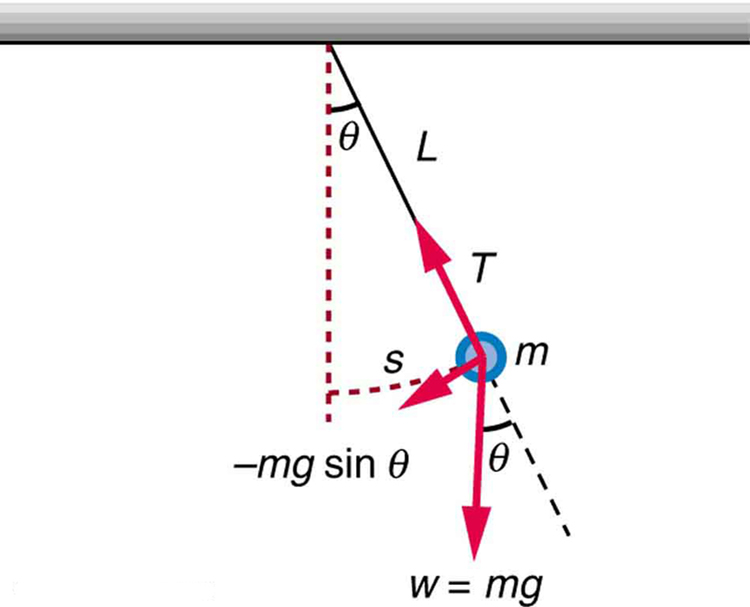
\includegraphics[width=.5\textwidth]{Figures_Part_3/pendulum.jpg}
\end{figure}
Using Newton's second law, we have that the force is equal to the mass times acceleration which leads us to the differential equation
\[
mL\theta'' = -mg\sin \theta. 
\]
This can be well approximated by using the first order approximation for $\sin \theta$. That is, we let
\[
\sin \theta \approx \theta
\]
to arrive at the differential equation
\[
\theta '' = -\frac{g}{L} \theta,
\]
which is the harmonic oscillator equation with $\omega^2 = \frac{g}{L}$. 
\end{ex}

\begin{exercise}
What is the solution to the above approximation of the pendulum equation?
\end{exercise}

\begin{ex}{Classical Diatomic Vibration}{classical_diatomic_vibration}
The Morse potential models the attraction between nuclei in a diatomic molecule.  Specifically, the potential is given by
\[
V(R)=D_e \left[ 1- e^{-a(R-R_e)}\right]^2.
\]
Here, $R$ is the distance between nuclei, $R_e$ is the equilibrium distance, $D_e$ is the dissociation energy of the molecule, and $a$ is a constant.  Stable molecules in low energy states only make small displacements $R-R_e$ from equilibrium and thus we can expand $V(R)$ in a series by
\begin{align*}
V(R) &= D_e\left[ a^2(R-R_e)^2-a^3(R-R_e)^3+\cdots \right]\\
&\approx a^2 D_e(R-R_e)^2.
\end{align*}
Then, Newton's second law with a potential is given by
\[
F= - \frac{dV}{dR}
\]
and so 
\[
F\approx -2a^2 D_e(R-R_e).
\]
Letting $x=(R-R_e)$ and $\omega^2 = \frac{2a^2D_e}{m}$, we have the differential equation
\begin{align*}
    x'' = -\omega^2 x
\end{align*}
which is again the simple harmonic oscillator.
\end{ex}

\begin{exercise}
Verify that the expansion of $V(R)$ about the point $R-R_e$ above is correct.
\end{exercise}

\section{Power Series Solutions to Differential Equations}

Power series provided a tool to approximate functions in order to simplify differential equations, but they also provide a way to solve differential equations as well.  It is in fact very close to the method of undetermined coefficients. The major difference is we (essentially) have to solve for infinitely many coefficients.  We briefly touched on recursive sequences here, and we'll find that these appear here as well. That is to say, if we consider a function given by a power series
\[
f(x) = \sum_{n=0}^\infty a_n x^n
\]
then the $a_n$ coefficients tend to depend on one another.  There are a handful of important functions in physics derived from power series solutions to certain differential equations.  For example, we have Bessel functions, Legendre polynomials, and Laguerre polynomials.  Bessel functions are, for example, found in solving for the wave modes on a circular drum head.  Legendre polynomials are found when solving Laplace's equation in spherical coordinates (we have seen Laplace's equation and will see spherical coordinates in the sequel). Specifically, one sees this when solving for states for the electron in a hydrogen atom.  The Laguerre polynomials also arise in quantum mechanics for the radial states of the Hydrogen atom. Not to mention, if one uses the Morse potential in the Schr\"odinger equation, one will find solutions are forms of Laguerre polynomials.  

To begin, it's easiest to consider some more simple examples of power series solutions.  The two equations we will work with for now are the population growth or decay equation
\[
f'(x)=kf(x)
\]
and the harmonic oscillator equation
\[
f''(x)=-\omega^2 f(x).
\]
As we already know the solutions to this equation, we don't actually need to solve this equations this way.  But, it does provide us a few working examples before we move onto an equation like Legendre's equation. In general, the idea is to take the ansatz that 
\[
f(x) = \sum_{n=0}^\infty a_n x^n
\]
and to take the necessary derivatives of the series and plug it into the given differential equation.  From there, one is able to determine the coefficients $a_n$ which determines the function $f(x)$.  If we are given an initial value (values if the differential equation is higher than first order), then we can explicitly determine every $a_n$ exactly.  Let us see this in action.

\begin{ex}{Power Series Solution for the Population Model}{pop_model_series}
Consider the initial value problem 
\[
f'(x)=kf(x)
\]
with $f(0)=1$.  Then, we know the particular solution to this initial value problem is
\[
f(x)=e^{kx}
\]
which we can find by separation.  So, if power series solutions are to work, we should achieve the same particular solution. We take the ansatz that
\[
f(x) = \sum_{n=0}^\infty a_n x^n
\]
which we can take a derivative of
\[
f'(x) = \sum_{n=1}^\infty na_n x^{n-1}.
\]
Now, we can plug both into our differential equation
\[
\sum_{n=1}^\infty na_n x^{n-1} = k \sum_{n=0}^\infty a_n x^n.
\]
It's usually easier to write out the terms in the series a bit so that we can match them.  So we have
\begin{align*}
    a_1 + 2a_2 x + 3 a_3 x^2 + 4 a_4 x^3 + \cdots &= k(a_0 + a_1 x + a_2 x^2 + a_3 x^3+ \cdots ).
\end{align*}
From this, we can see that we have
\begin{align*}
    a_1 &= k a_0\\
    a_2 &= \frac{k}{2} a_1\\
    a_3 &= \frac{k}{3} a_2 \\
    a_4 &= \frac{k}{4} a_3 \\
    &\cdots \\
    a_n &= \frac{k}{n} a_{n-1}.
\end{align*}
Let us also use our initial condition that $f(0)=1$, which means
\begin{align*}
    1=f(0)&=\sum_{n=0}^\infty a_n 0^n\\
    \implies~1&= a_0.
\end{align*}
Now, we can plug this into our above expressions for the coefficients which gives us
\begin{align*}
    a_1 &= k \\
    a_2 &= \frac{k^2}{2!} \\
    a_3 &= \frac{k^3}{3!}  \\
    a_4 &= \frac{k^4}{4!} \\
    &\vdots \\
    a_n &= \frac{k^n}{n!}.
\end{align*}
This gives us the particular solution
\begin{align*}
f(x) &= \sum_{n=0}^\infty \frac{k^n}{n!} x^n\\
&= \sum_{n=0}^\infty \frac{(kx)^n}{n!}\\
&= e^{kx}.
\end{align*}
Thus we have found exactly what we expected!
\end{ex}

\begin{exercise}
Carefully go through each step above and work out any details you feel are missing.
\end{exercise}

\begin{ex}{Power Series Solution for the Harmonic Oscillator}{power_series_for_harmonic_oscillator}
Consider the differential equation
\[
f''(x) = -\omega^2 f(x).
\]
We wish to find the general solution via a power series solution. We already know the general solution for this equation is of the form
\[
f(x)=C_1 \cos(\omega x)+C_2 \sin(\omega x)
\]
and so we should verify the power series allow us to find the same general solution.  So, we have the power series ansatz
\[
f(x) = \sum_{n=0}^\infty a_n x^n
\]
and thus
\begin{align*}
    f'(x) &= \sum_{n=1}^\infty na_n x^{n-1}\\
    f''(x)&= \sum_{n=2}^\infty n(n-1) x^{n-2}.
\end{align*}
We then plug in $f(x)$ and $f''(x)$ to the differential equation to get
\[
\sum_{n=2}^\infty n(n-1)a_n x^{n-2} = -\omega^2 \sum_{n=0}^\infty a_n x^n.
\]
Once again, I believe it is helpful to write out some of the terms of the series
\begin{align*}
    2a_2 +6a_3 x + 12 a_4 x^2 + 20 a_5 x^3 + \cdots &= \omega^2 (a_0 + a_1 x + a_2 x^2 + a_3 x^3 + \cdots ).
\end{align*}
This gives us the equations
\begin{align*}
a_2 &= \frac{-\omega^2}{2} a_0\\
a_3 &= \frac{-\omega^2}{6} a_1\\
a_4 &= \frac{-\omega^2}{12} a_2\\
a_5 &= \frac{-\omega^2}{20} a_3.
\end{align*}
Then we can determine the even coefficients $a_{2n}$ in terms of $a_0$ and the odd coefficients $a_{2n+1}$ in terms of $a_1$.  So we have
\begin{align*}
    a_2 &= \frac{-\omega^2}{2} a_0 &&& a_3 &= \frac{-\omega^2}{6} a_1\\
    a_4 &= \frac{\omega^4}{24} a_0 &&& a_5 &= \frac{\omega^4}{120} a_1\\
    &\vdots &&& &\vdots\\
    a_{2n} &= \frac{(-1)^n\omega^{2n}}{(2n)!}a_0 &&& a_{2n+1} &= \frac{(-1)^n\omega^{2n}}{(2n+1)!} a_1.
\end{align*}
Hence, the solution to the differential equation can be written as an even power series plus an odd power series as
\begin{align*}
    f(x)&= a_0 \sum_{n=0}^\infty \frac{\omega^{2n}}{(2n)!}x^{2n} + \frac{a_1}{\omega} \sum_{n=0}^\infty \frac{\omega^{2n+1}}{(2n+1)!} x^{2n+1}.
\end{align*}
If we rename $C_1 = a_0$ and $C_2 = \frac{a_1}{\omega}$ then we have
\begin{align*}
    f(x)&=C_1 \sum_{n=0}^\infty \frac{(\omega x)^{2n}}{(2n)!} + C_2 \sum_{n=0}^\infty \frac{(\omega x)^{2n+1}}{(2n+1)^1}\\
    &= C_1 \cos(\omega x)+C_2 \sin(\omega x).
\end{align*}
Again, we found exactly what we needed from the power series ansatz. Notice I made the substitution that $C_2=\frac{a_1}{\omega}$. This made the functions come out to being exactly what we want.  This is fine to do since $a_1$ is undetermined, so $\frac{a_1}{\omega}$ is undetermined as well.
\end{ex}

\begin{exercise}
Again, verify each step in the above solution and fill in any work you need.
\end{exercise}

\section{Orthogonal Polynomials from Power Series Solutions}

Throughout physics and chemistry there are equations that arise again and again.  A prime example would be the simple harmonic oscillator equation.  It would be a reasonable thought to believe that any oscillating system could be approximated by a harmonic oscillator.  There are of course other types of systems that will continue to pop their heads out in new ways.

We have solved some boundary value problems in 1-dimensional space, but when moving to higher dimensions, especially, when dealing with a specific geometry such as a rectangle, circle, disk, cylinder, or sphere for example, new equations begin to appear. It seems that the underlying geometry is very important for these boundary value problems. In fact, different geometrical objects may not even have a boundary! Take for example the unit circle which is the set of all points 
\[
\textrm{Unit Circle} = \left\{ e^{i \theta} ~|~ \theta \in [0,2\pi]\right\}.
\]
There is in fact no boundary for this shape. If you imagine walking along a circle, you'll never find the end of it.

\subsection{Legendre's Equation}

Eventually, we will try to understand the quantum mechanical solution to the hydrogen atom problem.  In the sequel, we build up the ability to do calculus in multiple dimensions and will solve some partial differential equations in higher dimensions.  Blackboxing some notation and terminology for now, the Schr\"odinger equation that describes the electron orbiting a proton (i.e., a hydrogen atom) has the Hamiltonian
\[
H=-\frac{\hbar^2}{2\mu} \nabla^2 - \frac{Ze^2}{4\pi \epsilon_0 r}
\]
where $r$ is the radial coordinate in the spherical coordinate system.  Recall Schr\"odinger's equation is then
\[
H\Psi(r,\theta, \phi) = E\Psi(r, \theta, \phi),
\]
where $r,\theta,\phi$ are the three spherical coordinates. The above equation turns out to be solvable using separation of variables, and the equation for the polar angle $\Theta(\theta)$ turns out to be
\[
\frac{\sin \theta}{\Theta} \frac{d}{d\theta}\left( \sin \theta \frac{d\Theta}{d\theta}\right) +A \sin^2 \theta - B = 0.
\]
If one takes the change of variables $P(\cos \theta)$ with $x=\cos \theta$ then the equation reads
\[
(1-x^2)\frac{d^2P}{dx^2}-2x\frac{dP}{dx}+\left(A-\frac{m^2}{1-x^2}\right)P=0.
\]
This is the \boldgreen{associated Legendre's equation}.  This equation turns out to be a bit more involved than \boldgreen{Legendre's equation} which is given by
\[
(1-x^2)f''(x)-2xf'(x)+m(m+1)f(x)=0.
\]
We will solve Legendre's equation instead.  

\subsubsection{Solving Legendre's Equation}

Legendre's equation arises from boundary value problems. Specifically, we have
\[
(1-x^2)f''(x)-2xf'(x)+m(m+1)f(x)=0,
\]
where we allow $x$ to be in the region $\Omega = [-1,1]$ and force $m$ to be a non-negative integer $m=0,1,2,3,\dots$.  The fact $m$ takes on just those values is that, for example, other requirements in the other variables present in Schr\"odinger's equation place a restriction on $m$. The parameter $m$ being restricted to non-negative integers is once again an example of quantization.  If we relate this differential equation to the true physics, this is saying that we have a discrete amount allowed states in the system.  We've seen this before with the particle in the 1-dimensional box.  We will also require the solutions to this equation for any $m$ to be \emph{normalized}. This is defined below, but in essence it is the requirement that the integral of each of the solution functions (for each $m$) is finite (and in fact equal to one).  This solves the problem uniquely for each $m$.

Much of the above is extra detail that one will eventually spend more time analyzing. For now, we want to solve this equation and we take the ansatz that $f(x)$ can be written as a power series
\[
f(x)=\sum_{n=0}^\infty a_n x^n.
\]
Then we can take the necessary derivatives
\begin{align*}
    f'(x)&=\sum_{n=1}^\infty na_n x^{n-1}\\
    f''(x)&= \sum_{n=2}^\infty n(n-1) a_n x^{n-2}.
\end{align*}
We can plug this into Legendre's equation to get
\begin{align*}
    (1-x^2)f''(x)-2xf'(x)+m(m+1)f(x)&=0\\
    (1-x^2)\sum_{n=2}^\infty n(n-1)a_n x^{n-2} - 2x \sum_{n=1}^\infty na_n x^{n-1} +m(m+1) \sum_{n=0}^\infty a_n x^n &=0\\
    \sum_{n=2}^\infty n(n-1) a_n x^{n-2} - \sum_{n=2}^\infty n(n-1)a_n x^n -\sum_{n=1}^\infty 2n a_n x^{n}+\sum_{n=0}^\infty m(m+1)a_n x^n &=0. 
\end{align*}
It is helpful to reindex the sums here to have all the powers of $x$ be the same so that we can relate each term slightly easier. So we have
\begin{align*}
    \sum_{n=0}^\infty (n+2)(n+1) a_{n+2} x^n - \sum_{n=2} n(n-1) a_n x^n - \sum_{n=1}^\infty 2na_n x^n +\sum_{n=0}^\infty m(m+1)a_n x^n &=0.
\end{align*}
Then if we make all the starting terms agree as well we have
\begin{align*}
    0&= \sum_{n=0}^1 (n+2)(n+1)a_{n+2}x^n -\sum_{n=1}^1 2na_n x^n +\sum_{n=0}^1
    m(m+1)a_n x^n\\
    &\quad + \sum_{n=2}^\infty \left[ (n+2)(n+1)a_{n+2}-n(n-1)a_n -2na_n +m(m+1)an\right]x^n.
\end{align*}
By setting the infinite sum equal to zero, we find $a_{n+2}$ in terms of $a_n$ by
\[
a_{n+2} = -\frac{(m-n)(m+n+1)}{(n+2)(n+1)}a_n.
\]
The finite sums above must also be zero and so
\begin{align*}
    0&= \sum_{n=0}^1 (n+2)(n+1)a_{n+2}x^n -\sum_{n=1}^1 2na_n x^n + \sum_{n=0}^\infty m(m+1)a_n x^n \\
    &= 2a_2 + 6a_3 x - 2a_1 x + m(m+1)a_0 + m(m+1) a_1 x\\
    &= (2a_2 +m(m+1)a_0)+(6a_3+(m(m+1)-2)a_1)x
\end{align*}
and thus we also have the equations
\begin{align*}
    a_2 &= \frac{m(m+1)}{2}a_0 &&& a_3 &= \frac{m(m+1)-2}{6}a_1\\
        &= \frac{m(m+1)}{2!} a_0 &&&  &= \frac{(m-1)(m+2)}{3!}a_1.
\end{align*}
We can thus solve for the even terms and odd terms from $a_0$ and $a_1$ respectively by
\begin{align*}
    a_{2n} &= (-1)^n \frac{m(m-2)\cdots (m-2n+2)(m+1)(m+3)\cdots (m+2n-1)}{(2n)!}a_0 &&& n&\geq 1\\
    a_{2n+1} &= (-1)^n \frac{(m-1)(m-3)\cdots(m-2n+1)(m+2)(m+4)\cdots (m+2n)}{(2n+1)!}a_1 &&& n&\geq 1.
\end{align*}
So for example, the first few even and first few odd terms are
\begin{align*}
    a_2 &= -\frac{m(m+1)}{2!}a_0 &&& a_3 &= -\frac{(m-1)(m+2)}{3!}a_1\\
    a_4 &= -\frac{m(m-2)(m+1)(m+3)}{4!} a_0 &&& a_5 &= \frac{(m-1)(m-3)(m+2)(m+4)}{5!}a_1.
\end{align*}
This splits up our solution into two linearly independent (even and odd) solutions by
\[
y_1(x)=\sum_{n=0}^\infty a_{2n}x^{2n} \qquad \textrm{and} \qquad y_2(x)=\sum_{n=0}^\infty a_{2n+1}x^{2n+1}.
\]

We then have a polynomial for every choice of $m$ we make.  We will denote these polynomials by $f_m(x)$. For example, notice if we take $m=0$, then we have $a_{2k}=0$ for $k\geq 1$ and so we have that $y_1(x)=a_0$. For this case $y_2(x)$ will not converge unless $a_1=0$.  Thus, when $m=0$ we have the polynomial
\[
f_0(x) = a_0. 
\]
If we take $m=1$, then we find that $a_{2k+1}=0$ for $k\geq 1$ and $y_1(x)$ diverges unless $a_0=0$.  Then we have
\[
f_1(x)= a_1 x.
\]
We can continue this process to find, for example,
\[
f_2(x)=a_0(1-3x^2) \qquad \textrm{and} \qquad f_3(x) = a_1\left( x - \frac{5x^3}{3}\right).
\]
There is a polynomial for each $m$, but I have only listed a few here.

\subsubsection{Orthogonality and Normalization}
It turns out that the polynomials created from this process are \boldgreen{orthogonal} since
\[
\int_{-1}^1 f_i(x)f_j(x)dx = 0
\]
when $i\neq j$.  Previously we saw a relationship like this when we studied a particle in the 1-dimensional box.  The idea is the same.  Since we have the undetermined constants $a_0$ and $a_1$ present for each polynomial (where each is also attached to a different value of $m$), we can \boldgreen{normalize} the polynomials above by requiring that
\[
\int_{-1}^1 |f_i(x)|^2 dx = 1.
\]
In doing this process, we find that the normalize polynomials are
\begin{align*}
    f_0(x)&=\sqrt{\frac{1}{2}} &&& f_1(x)&=\sqrt{\frac{3}{2}} x\\
    f_2(x)&= \sqrt{\frac{5}{8}}(1-3x^2) &&& f_3(x)&=\sqrt{\frac{63}{8}}\left( x -\frac{5x^3}{3}\right).
\end{align*}
One could continue generating normalization constants for each polynomial.

We can then say that this set of normalized polynomials is \boldgreen{orthonormal} which means that
\[
\int_{-1}^1 f_i(x)f_j(x)dx = \delta_{ij} = \begin{cases} 1 & \textrm{if $i=j$}\\ 0 & \textrm{if $i\neq j$}\end{cases}.
\]
It turns out to be orthonormal polynomials that are most useful for us.  These polynmomials correspond to states for a quantum system, and thus they should accurately represent a probability. Hence, the normalization.  The fact that the polynomials are also orthogonal is important in quantum mechanics as well, but it is a topic we will revisit in the sequel. In the next part of this text, we discuss linear algebra where we begin to explore the concepts of vectors in more generality.  In that sense, these polynomials are vectors in a vector space.  It's just that the vector space here is infinite dimensional, and is a bit harder to deal with than the finite dimensional case.